\section{Motor de Corrente Contínua}
\label{sec:motor_ref_teo}
% Introduzir o que funcionamento básico de um motor CC
% deixar claro qual o tipo será apresentado/utilizado no trabalho (motor CC de campo magnético fixo e com "escova")
Como o próprio nome indica, os motores CC são acionados por uma fonte de corrente contínua. Esse tipo de motor é amplamente utilizado em diversas aplicações.

Ele é constituído basicamente pelo enrolamento de armadura, enrolamento de campo ou ímãs permanentes, comutador e as escovas, onde:

\begin{itemize}
    \item Enrolamento de armadura: é localizado na parte giratória do motor de CC (rotor) que é responsável por produzir o torque que o movimenta, bem como a tensão de saída quando em modo de gerador.
    
    \item Enrolamento de campo: parte fixa responsável pelo fluxo magnético constante que irá atravessar a armadura. Em motores CC de pequenas dimensões, como os utilizados neste trabalho, o enrolamento de campo muitas vezes é substituído pela colocação de ímãs permanentes ao redor da armadura, responsáveis por gerar um campo magnético constante.
    
    \item Comutador: Possui a função de manter a corrente da armadura circulando no mesmo sentido, fazendo com que o torque mantenha seu sentido para uma tensão de entrada constante.
    
    \item Escovas: é por onde acontece o contato do enrolamento de armadura com a fonte de alimentação.
\end{itemize}


As máquinas de corrente contínua são bastante utilizadas em sistemas de controle em razão do seu comportamento essencialmente linear. O diagrama esquemático de uma máquina (motor ou gerador) CC é mostrado na figura \ref{fig:modelo_motor_dc}. O enrolamento de campo tem resistência $R_f$ e indutância $L_f$ e o enrolamento de armadura tem resistência $R_a$ e indutância $L_a$. As correntes e tensões nos enrolamentos de campo e de armadura $i_f$, $v_f$, $i_a$ e $v_a$, respectivamente. A tensão induzida na armadura é $v_g$. O torque e a velocidade angular no eixo do rotor são $\tau$ e $\omega$, respectivamente.

A tensão induzida no enrolamento de armadura é dada por:

\begin{equation}
    v_g = K_{1}\phi\omega
\end{equation}

E o torque é dado por:

\begin{equation}
    \tau = K_{1} \phi i_a 
\end{equation}onde $K_1$ é um parâmetro determinado pela estrutura física da máquina e $\phi$ é o fluxo magnético. Supondo que a máquina esteja operando na zona linear (ou seja, que o núcleo não esteja saturado), o fluxo é dado pela equação:
\begin{equation}
    \phi = K_{2}i_f
\end{equation}onde $K_2$ é uma constante e depende das características magnéticas do núcleo e do enrolamento de campo. No caso de motores com ímãs permanentes, o fluxo $\phi = \phi_\text{const}$ é constante, determinado pelos materiais e características de construção dos ímãs.

Motores geram potência mecânica, de forma que a velocidade de rotação $\omega$ é o sinal de saída e a tensão $v_a$ aplicada é o sinal de entrada. 

\begin{figure}[H]
    \centering
    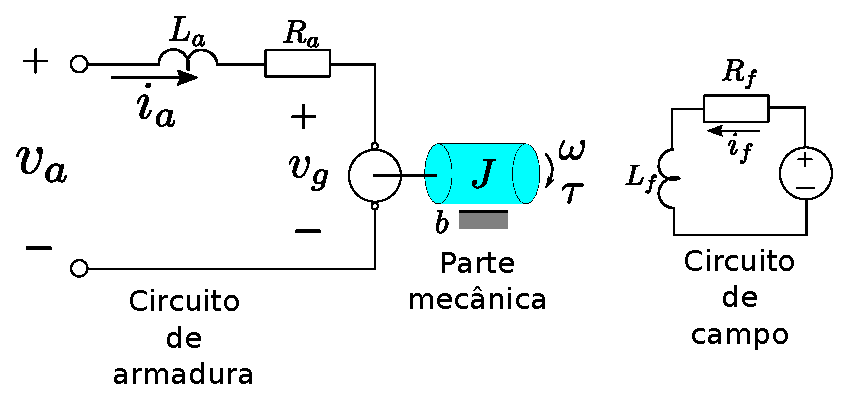
\includegraphics[width=0.5\textwidth]{figuras/ilustracoes/esquematico_motor_dc.eps}
    \caption{Diagrama esquemático de um motor CC.}
    \label{fig:modelo_motor_dc}
    \fonte{Própria.}
\end{figure}


A Figura \ref{fig:modelo_motor_dc} apresenta o diagrama esquemático para um motor de corrente contínua (CC) controlado pela armadura, ou seja, o sinal de entrada é a tensão aplicada na armadura ($v_a$). Nesse diagrama a carga está sendo modelada por um momento de inércia $J$ e um atrito viscoso de coeficiente $b$.

\begin{align*}
    v_g &= K_{1}\phi\omega= K_{1}K_{2}i_{f}\omega = K_{m}\omega\\
    \tau &= K_{1} \phi i_{a}= K_{1} K_{2}i_{f} i_{a} = K_{m}i_{a}
\end{align*}

A constante $K_{m}$ é conhecida como a constante do motor. Devido à relação apresentada anteriormente é possível modelar o circuito equivalente do motor CC como na imagem \ref{fig:eq_eletrico_motorcc}.
% figura baseada na fig. do livro texto da disciplina de modelagem.
\begin{figure}[H]
    \centering
    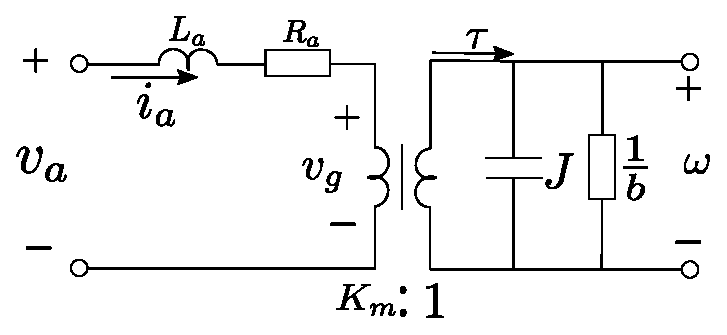
\includegraphics[width=0.6\textwidth]{figuras/ilustracoes/circuito_equivalente_motor_cc.eps}
    \caption{Equivalente elétrico de um motor CC}
    \label{fig:eq_eletrico_motorcc}
    \fonte{Própria.}
\end{figure}

Do circuito da figura \ref{fig:eq_eletrico_motorcc} extrai-se a seguinte função de transferência:

\begin{equation*}
    \frac{\Omega(s)}{V_a(s)} = \frac{K_m}{JL_{a}s^2 + \left(JR_a + BL_a \right)s + BR_a + K_{m}^2} \left[\frac{ rad.s^{-1}}{V}  \right]
\end{equation*}

Caso a impedância da armadura seja desprezada $(L_a \xrightarrow{} 0)$, o que quase sempre é possível pois a constante de tempo relacionada ao comportamento mecânico do motor é muito maior do que a relacionada ao funcionamento elétrico:

\begin{equation}
    \frac{\Omega(s)}{V_{a}(s)} = \frac{K_m}{JR_{a}s + BR_{a} + K_{m}^2} = \frac{K}{T_{m}s + 1} \left[\frac{ rad.s^{-1}}{V}  \right]
    \label{eq:motor_transf_func}
\end{equation}

Portando, caso a impedância da armadura seja desprezada, a função de transferência do motor que relaciona a velocidade angular com a tensão de entrada se comporta como a de um sistema de primeira ordem. A maior dificuldade encontrada ao se controlar motores CC é a amplitude elevada da corrente de armadura, o que requer a utilização de sinal $v_a$ de entrada fornecido por uma fonte de alta potência.